\section{Рабочий проект}
\subsection{Спецификация компонентов программной системы}

Можно выделить следующий список классов и их методов, использованных при разработке web-приложения (таблица \ref{class:rtable}). Пример таблицы с уменьшенным межстрочным интервалом.

\renewcommand{\arraystretch}{0.8} % уменьшение расстояний до сетки таблицы
\begin{xltabular}{\textwidth}{|l|X|}
\caption{Описание классов, используемых в веб-приложении\label{class:rtable}}\\
\hline \centrow Название класса & \centrow Описание класса\\
\hline \centrow 1 & \centrow 2\\ \hline
\endfirsthead
\caption*{Продолжение таблицы \ref{class:rtable}}\\
\hline \centrow 1 & \centrow 2\\ \hline
\finishhead
index.php & Основная веб-страница, отображающая интерактивную карту и элементы пользовательского интерфейса. Позволяет управлять фильтрами, маршрутами, добавлением объектов и аккаунтом. Подключает JavaScript-компоненты и карты Яндекса.\\
\hline add\_object.php & Обрабатывает отправку данных при добавлении новой точки. Сохраняет координаты, название, категорию и адрес в базу. Поддерживает модерацию.\\
\hline auth.php & Определяет текущий статус авторизации пользователя и возвращает результат в формате JSON.\\
\hline check\_favorite.php & Проверяет наличие определённого объекта в списке избранного пользователя. Возвращает булево значение в JSON.\\
\hline check-auth.php & Проверяет наличие активной пользовательской сессии. Используется для динамической загрузки элементов интерфейса в зависимости от статуса авторизации (например, отображение меню аккаунта). Возвращает ответ в формате JSON.\\
\hline data.php & Загружает данные о точках с учётом прав доступа. Отдаёт описание, изображения и категорию объектов.\\
\hline db.php & Содержит параметры подключения к базе данных и инициализирует PDO-соединение. Используется другими PHP-скриптами.\\
\hline delete\_route.php & Удаляет сохранённый маршрут из базы, предварительно проверяя авторизацию пользователя.\\
\hline functions.php & Набор вспомогательных функций для валидации данных форм, очистки ввода и отображения ошибок.\\
\hline get\_favorite\_points.php & Возвращает список точек, добавленных пользователем в избранное, включая координаты и названия.\\
\hline get\_favorite\_routes.php & Загружает маршруты из избранного, включая последовательность точек и тип маршрута.\\
\hline get\_point\_name.php & Определяет название объекта по его координатам. Применяется для генерации названий в маршрутах.\\
\hline get\_images.php & Загружает изображения, прикреплённые к определённой туристической точке. Возвращает массив ссылок на изображения, применяемый в карточке объекта и балуне.\\
\hline get\_reviews.php & Загружает все отзывы, связанные с конкретным объектом. Возвращает текст, авторов и даты.\\
\hline login.php & Осуществляет проверку введённого email и пароля. При успешной проверке инициирует сессию.\\
\hline logout.php & Завершает пользовательский сеанс, удаляя сессионные данные и перенаправляя на главную страницу.\\
\hline moderate.php & Интерфейс модерации для администраторов. Позволяет управлять статусом новых объектов, описаний и изображений.\\
\hline register.php & Регистрирует новых пользователей, проводит валидацию данных и сохраняет хешированный пароль.\\
\hline save\_object.php & Обрабатывает дополнительную информацию для объектов (описания, изображения). Поддерживает модерацию.\\
\hline save\_point.php & Добавляет или убирает точку из избранного. Возвращает результат действия.\\
\hline save\_route.php & Сохраняет маршрут в профиль пользователя: координаты точек, тип маршрута, название.\\
\hline send\_review.php & Добавляет отзыв к выбранному объекту. Проверяет авторизацию перед сохранением.\\
\hline addData.js & Отвечает за отправку данных при добавлении нового объекта. Проверяет авторизацию перед отправкой.\\
\hline addObject.js & Позволяет взаимодействовать с временной меткой на карте при добавлении объекта: перемещение, адрес.\\
\hline addObjectInformation.js & Управляет формой для добавления описания и изображений к существующему объекту.\\
\hline addObjectPicture.js & Реализует предпросмотр и удаление изображений перед отправкой.\\
\hline addReview.js & Обрабатывает отображение и отправку отзывов. Подгружает существующие отзывы с сервера.\\
\hline favoritePoint.js & Отвечает за добавление и удаление точек из избранного, а также обновление визуального состояния.\\
\hline Filter.js & Реализует фильтрацию точек на карте по выбранным категориям. Изменяет видимость меток.\\
\hline loadFavoritesPoints.js & Загружает избранные точки пользователя и отображает их на карте с возможностью удаления.\\
\hline loadFavoritesRoutes.js & Загружает маршруты из избранного и отображает их на карте. Обеспечивает удаление маршрутов.\\
\hline Location.js & Определяет текущие координаты пользователя через Geolocation API и отображает их на карте.\\
\hline openAccountMenu.js & Управляет открытием и скрытием меню аккаунта, включая вход, регистрацию и личный кабинет.\\
\hline openAddMenu.js & Отвечает за отображение меню добавления новых объектов на карту.\\
\hline openFilterMenu.js & Управляет отображением меню фильтрации объектов по категориям.\\
\hline openRegistrationMenu.js & Отвечает за форму регистрации, обрабатывает валидацию и отображение ошибок.\\
\hline openRouteMenu.js & Отображает меню построения маршрутов, управления точками и сохранения.\\
\hline routeHandler.js & Основной модуль маршрутизации. Строит и обновляет маршруты, рассчитывает расстояние и длительность.\\
\hline openObjectInformationMenu.js & Отвечает за отображение панели редактирования информации об объекте. Активирует форму добавления описания и изображений, а также подгружает текущие данные, если они уже существуют.\\
\hline openSearchMenu.js & Отвечает за открытие и закрытие панели поиска. Обрабатывает ввод поискового запроса пользователем, фокусирует поле ввода и управляет визуальной активностью панели. Интегрирован с фильтрацией или подсказками.\\
\end{xltabular}
\renewcommand{\arraystretch}{1.0} % восстановление сетки

\subsubsection{Спецификация файла routeHandler.js}

В таблице \ref{class:rtable1} представлены функции файла favoritePoint.js.

\renewcommand{\arraystretch}{0.8} % уменьшение расстояний до сетки таблицы
\begin{xltabular}{\textwidth}{|l|X|}
	\caption{Функции файла routeHandler.js\label{class:rtable1}}\\
	\hline \centrow Название функции & \centrow Описание функции\\
	\hline \centrow 1 & \centrow 2\\ \hline
	\endfirsthead
	\caption*{Продолжение таблицы \ref{class:rtable1}}\\
	\hline \centrow 1 & \centrow 2\\ \hline
	\finishhead
	setMapInstance(map) & Сохраняет экземпляр карты в переменную mapInstance для использования в других частях приложения.\\
	\hline setupRouteTypeButtons() & Назначает обработчики кнопок выбора типа маршрута (пеший, авто и др.). Обновляет активное состояние и перерисовывает маршрут при необходимости.\\
	\hline optimizeRoute() & Выполняет простую оптимизацию порядка точек маршрута на основе жадного алгоритма ближайшей точки.\\
	\hline getDistance(coords1, coords2) & Вычисляет расстояние между двумя координатами по формуле haversine. Используется в оптимизации маршрута.\\
	\hline toRad(degrees) & Преобразует градусы в радианы для расчёта расстояния между координатами.\\
	\hline attachRouteButtonHandler(coords, title) & Привязывает кнопку в балуне к добавлению точки в маршрут. Вызывает addRoutePoint.\\
	\hline addRoutePoint(coords, title) & Добавляет выбранную точку в маршрут. При первом добавлении определяет текущее местоположение как стартовую точку.\\
	\hline getPointNameFromDB(coords, callback) & Выполняет fetch-запрос к серверу для получения названия точки по координатам.\\
	\hline drawCustomRoute() & Строит маршрут на карте с использованием API Яндекс.Карт. Отображает данные о длине и времени маршрута, обновляет интерфейс.\\
	\hline formatTime(minutes) & Форматирует время маршрута в удобный вид: часы и минуты.\\
	\hline openRouteMenu() & Показывает меню управления маршрутом, если оно скрыто.\\
	\hline updateRouteListUI() & Обновляет список точек маршрута в интерфейсе на основе текущего состояния массива routePoints.\\
	\hline enableRouteListSorting() & Включает возможность перетаскивания и изменения порядка точек в маршруте.\\
	\hline getAddressesForRoutePoints() & Выполняет обратное геокодирование точек маршрута для отображения адресов.\\
	\hline setupResetButton() & Назначает обработчик на кнопку сброса маршрута. При нажатии очищает маршрут и интерфейс.\\
	\hline resetRoute() & Полностью удаляет текущий маршрут, очищает карту и связанные элементы интерфейса.\\
	\hline removeRoutePoint(index) & Удаляет точку из маршрута по индексу и перерисовывает маршрут.\\
	\hline setupRouteModalHandlers() & Назначает обработчики модального окна сохранения маршрута: открыть, закрыть, подтвердить.\\
	\hline showRouteNameModal() & Проверяет авторизацию и минимальное количество точек. Если условия соблюдены — показывает модальное окно для ввода названия маршрута.\\
	\hline hideRouteNameModal() & Скрывает модальное окно сохранения маршрута.\\
	\hline saveFavoriteRouteWithName() & Отправляет маршрут с названием на сервер для сохранения в избранное.\\
	\hline initInstructionsToggle() & Управляет видимостью блока пошаговых инструкций по маршруту. Назначает обработчик на кнопку переключения.\\
	\hline showNavigationInstructionsFromMultiRoute(route) & Извлекает сегменты маршрута из API Яндекс.Карт и формирует HTML-блок с пошаговыми указаниями.\\
	\hline setPointsInstance(points) & Сохраняет список всех точек в переменную allPoints для последующего анализа.\\
	\hline getOptimalCircularRoutePoints() & Строит кольцевой маршрут вокруг временной метки с заданной длиной, выбирая ближайшие точки до достижения лимита.\\
	\hline setupCircularRoute() & Назначает обработчик на кнопку построения кольцевого маршрута. Запускает процесс выбора оптимальных точек.\\
\end{xltabular}

\subsubsection{Спецификация файла addObject.js}

В таблице \ref{class:rtable2} представлены функции файла addObject.js.

\renewcommand{\arraystretch}{0.8} % уменьшение расстояний до сетки таблицы
\begin{xltabular}{\textwidth}{|l|X|}
	\caption{Функции файла addObject.js\label{class:rtable2}}\\
	\hline \centrow Название функции & \centrow Описание функции\\
	\hline \centrow 1 & \centrow 2\\ \hline
	\endfirsthead
	\caption*{Продолжение таблицы \ref{class:rtable2}}\\
	\hline \centrow 1 & \centrow 2\\ \hline
	\finishhead
	addPlacemark(map) & Создаёт на карте временную метку в центре экрана, которая может быть перемещена пользователем. При перемещении обновляет поля с адресом и координатами. Также назначает обработчик для удаления метки и очистки полей при закрытии панели добавления. Использует геокодирование для получения текстового адреса.\\
	\hline updateAddressAndCoordinates(coords) & Выполняет обратное геокодирование координат, получая адрес с помощью ymaps.geocode(). После получения адреса заполняет соответствующие поля формы: текстовый адрес и числовые значения широты и долготы. Используется для обновления данных при перемещении временной метки.\\
\end{xltabular}

\subsubsection{Спецификация файла addReview.js}

В таблице \ref{class:rtable3} представлены функции файла addReview.js.

\renewcommand{\arraystretch}{0.8} % уменьшение расстояний до сетки таблицы
\begin{xltabular}{\textwidth}{|l|X|}
	\caption{Функции файла addReview.js\label{class:rtable3}}\\
	\hline \centrow Название функции & \centrow Описание функции\\
	\hline \centrow 1 & \centrow 2\\ \hline
	\endfirsthead
	\caption*{Продолжение таблицы \ref{class:rtable3}}\\
	\hline \centrow 1 & \centrow 2\\ \hline
	\finishhead
	addReviewToList(review) & Добавляет переданный отзыв в начало списка на странице. Создаёт HTML-элемент <li>, форматирует дату отзыва и отображает его содержимое в пользовательском интерфейсе.\\
	\hline loadReviews(objectId) & Загружает отзывы с сервера по идентификатору объекта. Отображает список отзывов в интерфейсе или сообщение об отсутствии данных. В случае ошибки выводит сообщение о неудачной загрузке.\\
\end{xltabular}

\subsubsection{Спецификация файла favoritePoints.js}

В таблице \ref{class:rtable4} представлены функции файла favoritePoints.js.

\renewcommand{\arraystretch}{0.8} % уменьшение расстояний до сетки таблицы
\begin{xltabular}{\textwidth}{|l|X|}
	\caption{Функции файла favoritePoints.js\label{class:rtable4}}\\
	\hline \centrow Название функции & \centrow Описание функции\\
	\hline \centrow 1 & \centrow 2\\ \hline
	\endfirsthead
	\caption*{Продолжение таблицы \ref{class:rtable4}}\\
	\hline \centrow 1 & \centrow 2\\ \hline
	\finishhead
	attachFavoriteButtonHandler(pointId) & Назначает обработчик на кнопку «добавить в избранное» в балуне объекта. При клике выполняет добавление точки и обновление визуального состояния.\\
	\hline addToFavorites(pointId) & Асинхронно проверяет авторизацию пользователя и отправляет запрос на добавление/удаление точки из избранного. Возвращает результат действия.\\
	\hline loadFavoritePoints() & Загружает с сервера текущий список избранных точек пользователя и вызывает их отображение.\\
	\hline renderFavoritePoints(points) & Отрисовывает список избранных точек в интерфейсе. Назначает обработчики для перемещения к точке на карте и удаления из избранного.\\
	\hline removeFromFavorites(pointId, element, point) & Удаляет точку из избранного, обновляет интерфейс, повторно открывает балун при необходимости и показывает сообщение, если список стал пустым.\\
	\hline reopenBalloonForPoint(point) & Повторно открывает балун объекта на карте, если он был закрыт после обновления состояния избранного.\\
	\hline updateFavoriteButtonInBalloon(pointId, isFavorite) & Обновляет внешний вид кнопки «избранное» в балуне соответствующего объекта в зависимости от его текущего статуса.\\
	\hline focusPointOnMap(point) & Центрирует карту на координатах указанной точки и открывает её балун, если объект найден среди отображаемых.\\
\end{xltabular}

\subsubsection{Спецификация файла loadFavoritesRoutes.js}

В таблице \ref{class:rtable5} представлены функции файла loadFavoritesRoutes.js.

\renewcommand{\arraystretch}{0.8} % уменьшение расстояний до сетки таблицы
\begin{xltabular}{\textwidth}{|l|X|}
	\caption{Функции файла loadFavoritesRoutes.js\label{class:rtable5}}\\
	\hline \centrow Название функции & \centrow Описание функции\\
	\hline \centrow 1 & \centrow 2\\ \hline
	\endfirsthead
	\caption*{Продолжение таблицы \ref{class:rtable5}}\\
	\hline \centrow 1 & \centrow 2\\ \hline
	\finishhead
	loadFavoriteRoutes() & Загружает с сервера список маршрутов, сохранённых пользователем в избранное, и передаёт данные в функцию отрисовки.\\
	\hline renderFavoriteRoutes(routes) & Отображает полученные маршруты в интерфейсе. Создаёт элементы списка с названием и типом маршрута, кнопкой удаления и возможностью загрузки маршрута на карту.\\
	\hline getRouteTypeName(type) & Преобразует техническое обозначение типа маршрута (auto, pedestrian, masstransit) в человекочитаемый формат.\\
	\hline loadRouteToMap(route) & Загружает выбранный маршрут на карту. Создаёт стартовую точку и добавляет остальные, определяя для них имена через обратное геокодирование, затем строит маршрут.\\
	\hline getPointNameFromDB(coords, callback) & Выполняет запрос к серверу для получения названия объекта по его координатам. Вызывает переданный колбэк с результатом.\\
	\hline deleteFavoriteRoute(routeId) & Удаляет выбранный маршрут из избранного, отправляя запрос на сервер. При успешном удалении обновляет интерфейс и сбрасывает отображаемый маршрут, если он активен.\\
\end{xltabular}

\subsubsection{Спецификация файла loadFavoritesPoints.js}

В таблице \ref{class:rtable6} представлены функции файла loadFavoritesPoints.js.

\renewcommand{\arraystretch}{0.8} % уменьшение расстояний до сетки таблицы
\begin{xltabular}{\textwidth}{|l|X|}
	\caption{Функции файла loadFavoritesPoints.js\label{class:rtable6}}\\
	\hline \centrow Название функции & \centrow Описание функции\\
	\hline \centrow 1 & \centrow 2\\ \hline
	\endfirsthead
	\caption*{Продолжение таблицы \ref{class:rtable6}}\\
	\hline \centrow 1 & \centrow 2\\ \hline
	\finishhead
	constructor() & Вызывается при создании экземпляра класса. Запускает асинхронную инициализацию через метод init().\\
	\hline init() & Выполняет начальную загрузку избранных точек, вызывая loadFavoritePoints(). Обрабатывает возможные ошибки.\\
	\hline loadFavoritePoints() & Асинхронно получает список избранных точек пользователя с сервера. При успешном ответе передаёт данные в метод отображения.\\
	\hline renderFavoritePoints(points) & Отрисовывает список избранных точек в интерфейсе. Создаёт элементы списка, назначает обработчики кликов для фокусировки и удаления точек.\\
	\hline removeFavoritePoint(pointId, element, point) & Удаляет точку из избранного, отправляя запрос на сервер. Обновляет визуальное состояние списка и вызывает связанные обновления в балуне карты.\\
	\hline focusPointOnMap(point) & Центрирует карту на координатах выбранной точки и открывает её балун, если точка отображается на карте.\\
\end{xltabular}

\subsubsection{Спецификация файла Filter.js}

В таблице \ref{class:rtable7} представлены функции файла Filter.js.

\renewcommand{\arraystretch}{0.8} % уменьшение расстояний до сетки таблицы
\begin{xltabular}{\textwidth}{|l|X|}
	\caption{Функции файла Filter.js\label{class:rtable7}}\\
	\hline \centrow Название функции & \centrow Описание функции\\
	\hline \centrow 1 & \centrow 2\\ \hline
	\endfirsthead
	\caption*{Продолжение таблицы \ref{class:rtable7}}\\
	\hline \centrow 1 & \centrow 2\\ \hline
	\finishhead
	addObjectToList(point) & Добавляет объект в список на боковой панели фильтра. Включает название, категорию, адрес и кнопки: «Показать на карте» и «О объекте». Назначает обработчики для открытия балуна и подробной информации.\\
	\hline updateFilters() & Обновляет отображение объектов на карте и в списке в зависимости от выбранных категорий в фильтре. Управляет отображением и скрытием меток и формированием списка объектов.\\
	\hline initialize() & Проверяет наличие массива placemarks в window и, как только он доступен, вызывает updateFilters() для инициализации фильтрации объектов.\\
\end{xltabular}

\subsubsection{Спецификация файла Location.js}

В таблице \ref{class:rtable8} представлены функции файла Location.js.

\renewcommand{\arraystretch}{0.8} % уменьшение расстояний до сетки таблицы
\begin{xltabular}{\textwidth}{|l|X|}
	\caption{Функции файла Location.js\label{class:rtable8}}\\
	\hline \centrow Название функции & \centrow Описание функции\\
	\hline \centrow 1 & \centrow 2\\ \hline
	\endfirsthead
	\caption*{Продолжение таблицы \ref{class:rtable8}}\\
	\hline \centrow 1 & \centrow 2\\ \hline
	\finishhead
	initLocationToggle(mapInstance) & Инициализирует переключатель отображения текущего местоположения пользователя. При нажатии на кнопку запускает или останавливает отслеживание координат через navigator.geolocation.watchPosition. Создаёт и обновляет метку на карте с координатами пользователя.\\
\end{xltabular}

\subsection{Модульное тестирование программной системы}

Процесс разработки программного обеспечения невозможен без всесторонней проверки работоспособности реализованных компонентов. Одним из ключевых этапов обеспечения надёжности системы является модульное тестирование, целью которого становится изолированная проверка отдельных функций и классов на корректность выполнения предусмотренных задач.

В рамках реализации веб-приложения для отображения туристических объектов и построения маршрутов особое внимание уделяется логике взаимодействия с географическими данными: вычислению расстояний, сортировке точек, формированию маршрутов, а также вспомогательным преобразованиям данных. Для оценки корректности работы таких модулей разработаны и проведены модульные тесты с использованием языка Python и библиотеки unittest.

Применение модульного тестирования позволяет выявлять логические ошибки на ранних этапах, минимизировать риски при изменениях в коде, а также служит основой для будущего расширения функциональности. В данной главе представлены примеры тестирования ключевых компонентов, участвующих в построении маршрутов и обработке пользовательских данных, с пояснением логики их функционирования и анализа результатов выполнения.

Модульный тест для класса User из модели данных представлен на рисунке \ref{unitUser:rimage}.

\begin{figure}[H]
\begin{lstlisting}[language=Python]
import unittest
import math

# Прототипы функций, эквивалентных тем, что есть в routeHandler.js

def to_rad(degrees):
	return degrees * (math.pi / 180)

def get_distance(coords1, coords2):
	lat1, lon1 = coords1
	lat2, lon2 = coords2
	R = 6371  # Радиус Земли в км
	
	d_lat = to_rad(lat2 - lat1)
	d_lon = to_rad(lon2 - lon1)
	
	a = math.sin(d_lat / 2) ** 2 + math.cos(to_rad(lat1)) * math.cos(to_rad(lat2)) * math.sin(d_lon / 2) ** 2
	c = 2 * math.atan2(math.sqrt(a), math.sqrt(1 - a))
	
	return R * c

def format_time(minutes):
	hours = minutes // 60
	mins = minutes % 60
	if hours > 0:
		return f"{hours} ч {mins} мин"
	return f"{mins} мин"

def optimize_route(route_points):
	if len(route_points) <= 1:
		return route_points
	
	optimized = [route_points[0]]
	remaining = route_points[1:]
	
	while remaining:
		last = optimized[-1]
		closest = min(remaining, key=lambda p: get_distance(last['coords'], p['coords']))
		optimized.append(closest)
		remaining.remove(closest)
	
	return optimized


class TestRouteHandler(unittest.TestCase):

	def test_to_rad(self):
		self.assertAlmostEqual(to_rad(180), math.pi)
		self.assertAlmostEqual(to_rad(0), 0)
	
	def test_get_distance(self):
		coords1 = [51.7347, 36.1907]
		coords2 = [51.7357, 36.1917]
		distance = get_distance(coords1, coords2)
		self.assertTrue(0 < distance < 1)  # Ожидаем менее 1 км
	
	def test_format_time(self):
		self.assertEqual(format_time(45), "45 мин")
		self.assertEqual(format_time(125), "2 ч 5 мин")
	
	def test_optimize_route(self):
		route = [
			{'coords': [51.7347, 36.1907]},
			{'coords': [51.7357, 36.1917]},
			{'coords': [51.7367, 36.1927]},
		]
		optimized = optimize_route(route)
		self.assertEqual(len(optimized), 3)
		self.assertEqual(optimized[0], route[0])
		self.assertIn(route[1], optimized)
		self.assertIn(route[2], optimized)


if __name__ == '__main__':
unittest.main()

\end{lstlisting}  
\caption{Модульный тест файла routeHandler.js}
\label{unitUser:rimage}
\end{figure}

\subsection{Системное тестирование программной системы}

После реализации всех ключевых компонентов веб-приложения необходимо убедиться в целостности и согласованной работе системы в условиях, приближенных к реальной эксплуатации. Для этих целей проводится системное тестирование — этап, на котором проверяется функционирование всего программного комплекса в целом, включая как отдельные модули, так и их взаимодействие между собой.

Системное тестирование охватывает пользовательские сценарии — от отображения карты и взаимодействия с объектами до построения маршрутов, работы с фильтрами, регистрацией, авторизацией и сохранением пользовательских данных. В ходе данного этапа особое внимание уделяется корректности отклика интерфейса, устойчивости системы к ошибкам, точности географических вычислений, а также доступности всех предусмотренных функций.

Тестирование проводится в условиях, максимально приближенных к эксплуатации: через пользовательский интерфейс, с имитацией различных действий пользователей и переключением режимов отображения. Результатом системного тестирования становится подтверждение того, что приложение выполняет все заявленные функции корректно, логически согласовано и соответствует ожиданиям пользователей.

На рисунке \ref{r1:image} представлена главная страница веб-приложения.

%\newpage % при необходимости можно переносить рисунок на новую страницу
\begin{figure}[H] % H - рисунок обязательно здесь, или переносится, оставляя пустоту
\center{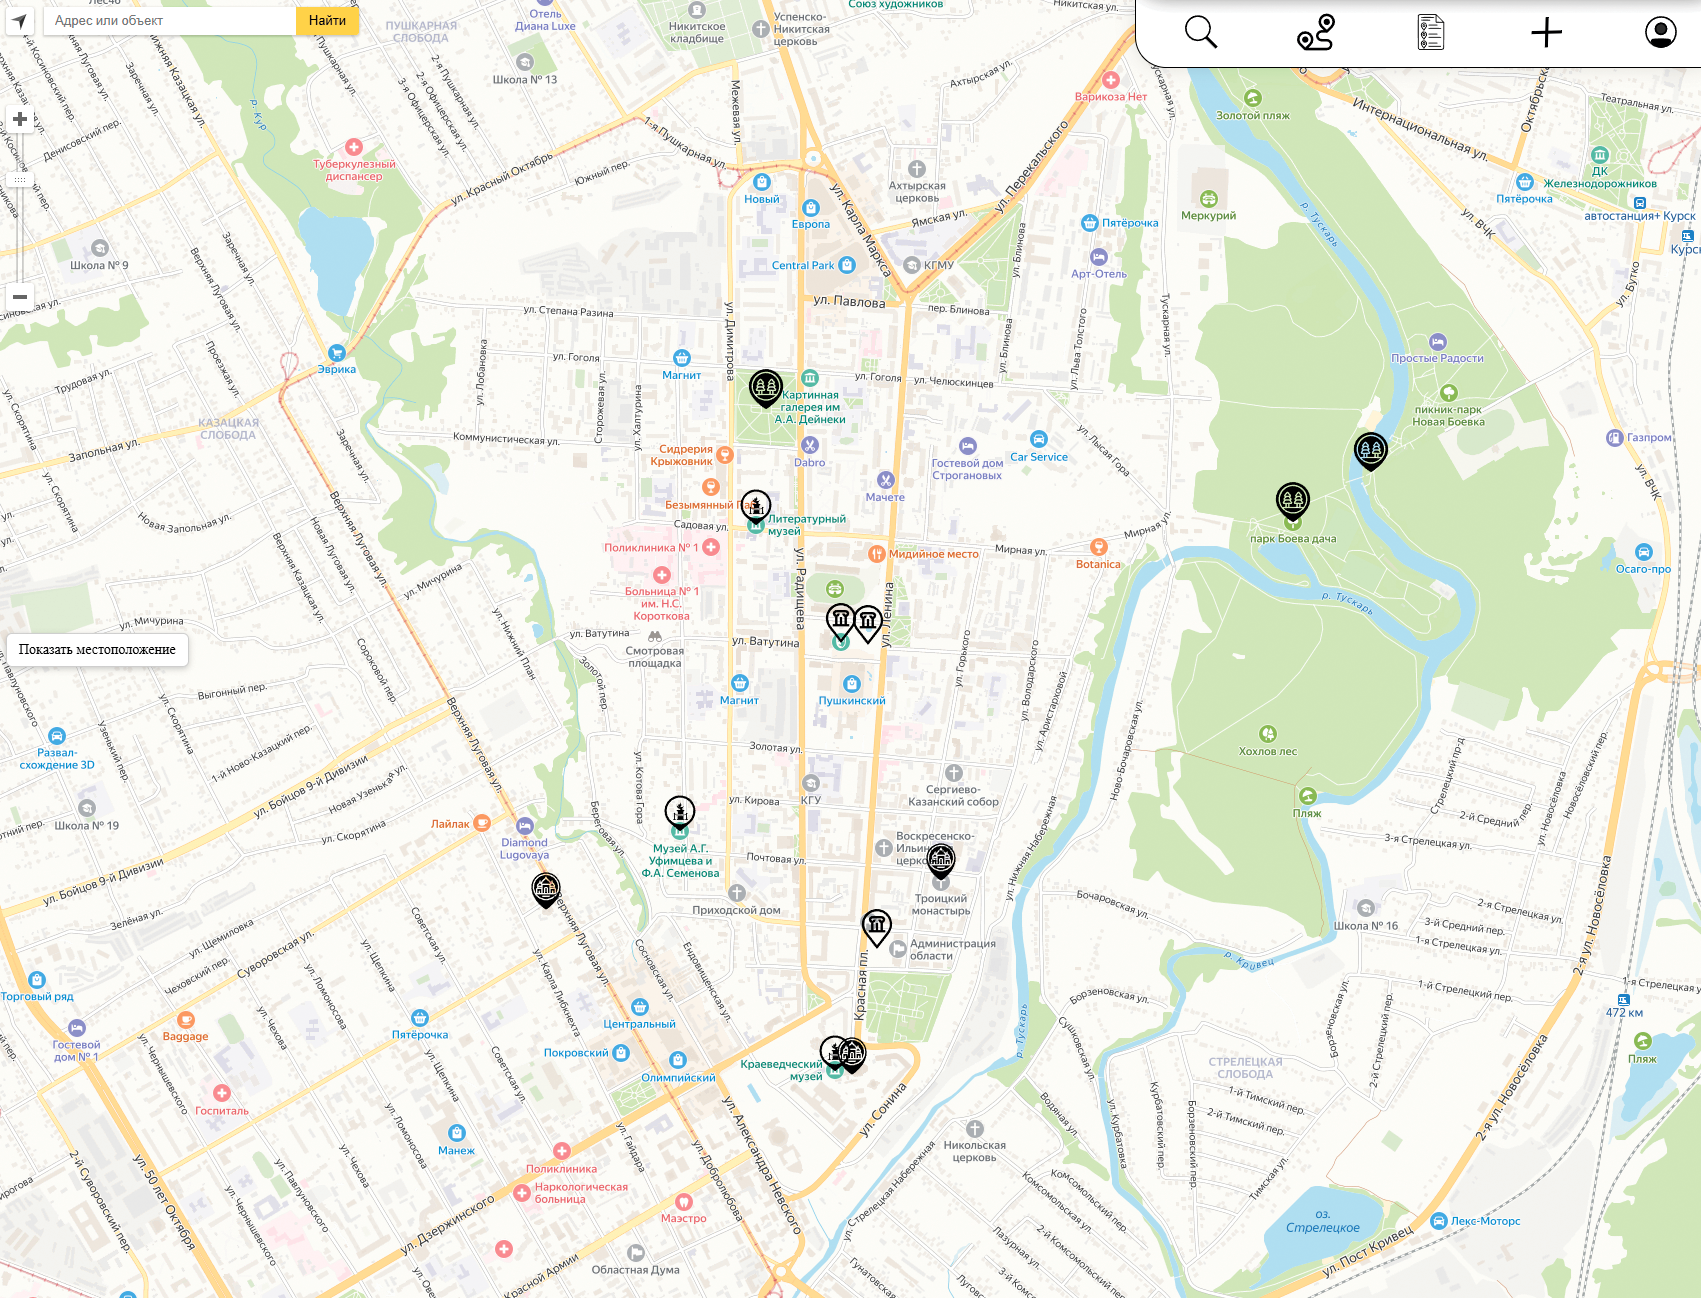
\includegraphics[width=1\linewidth]{r1}}
\caption{Главная страница веб-приложения}
\label{r1:image}
\end{figure}

\newpage
На рисунке \ref{r2:image} представлен поиск туристического объекта по названию.

\begin{figure}[H]
\center{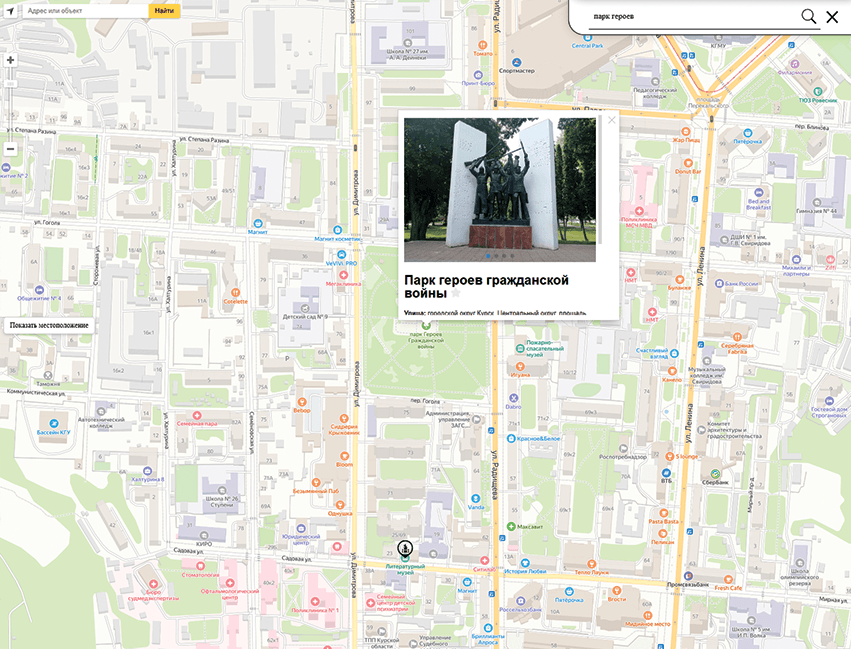
\includegraphics[width=1\linewidth]{r2}}
\caption{Поиск туристического объекта по названию}
\label{r2:image}
\end{figure}

\newpage
На рисунке \ref{r3:image} представлен составленный пользователем маршрут.

\begin{figure}[H]
\center{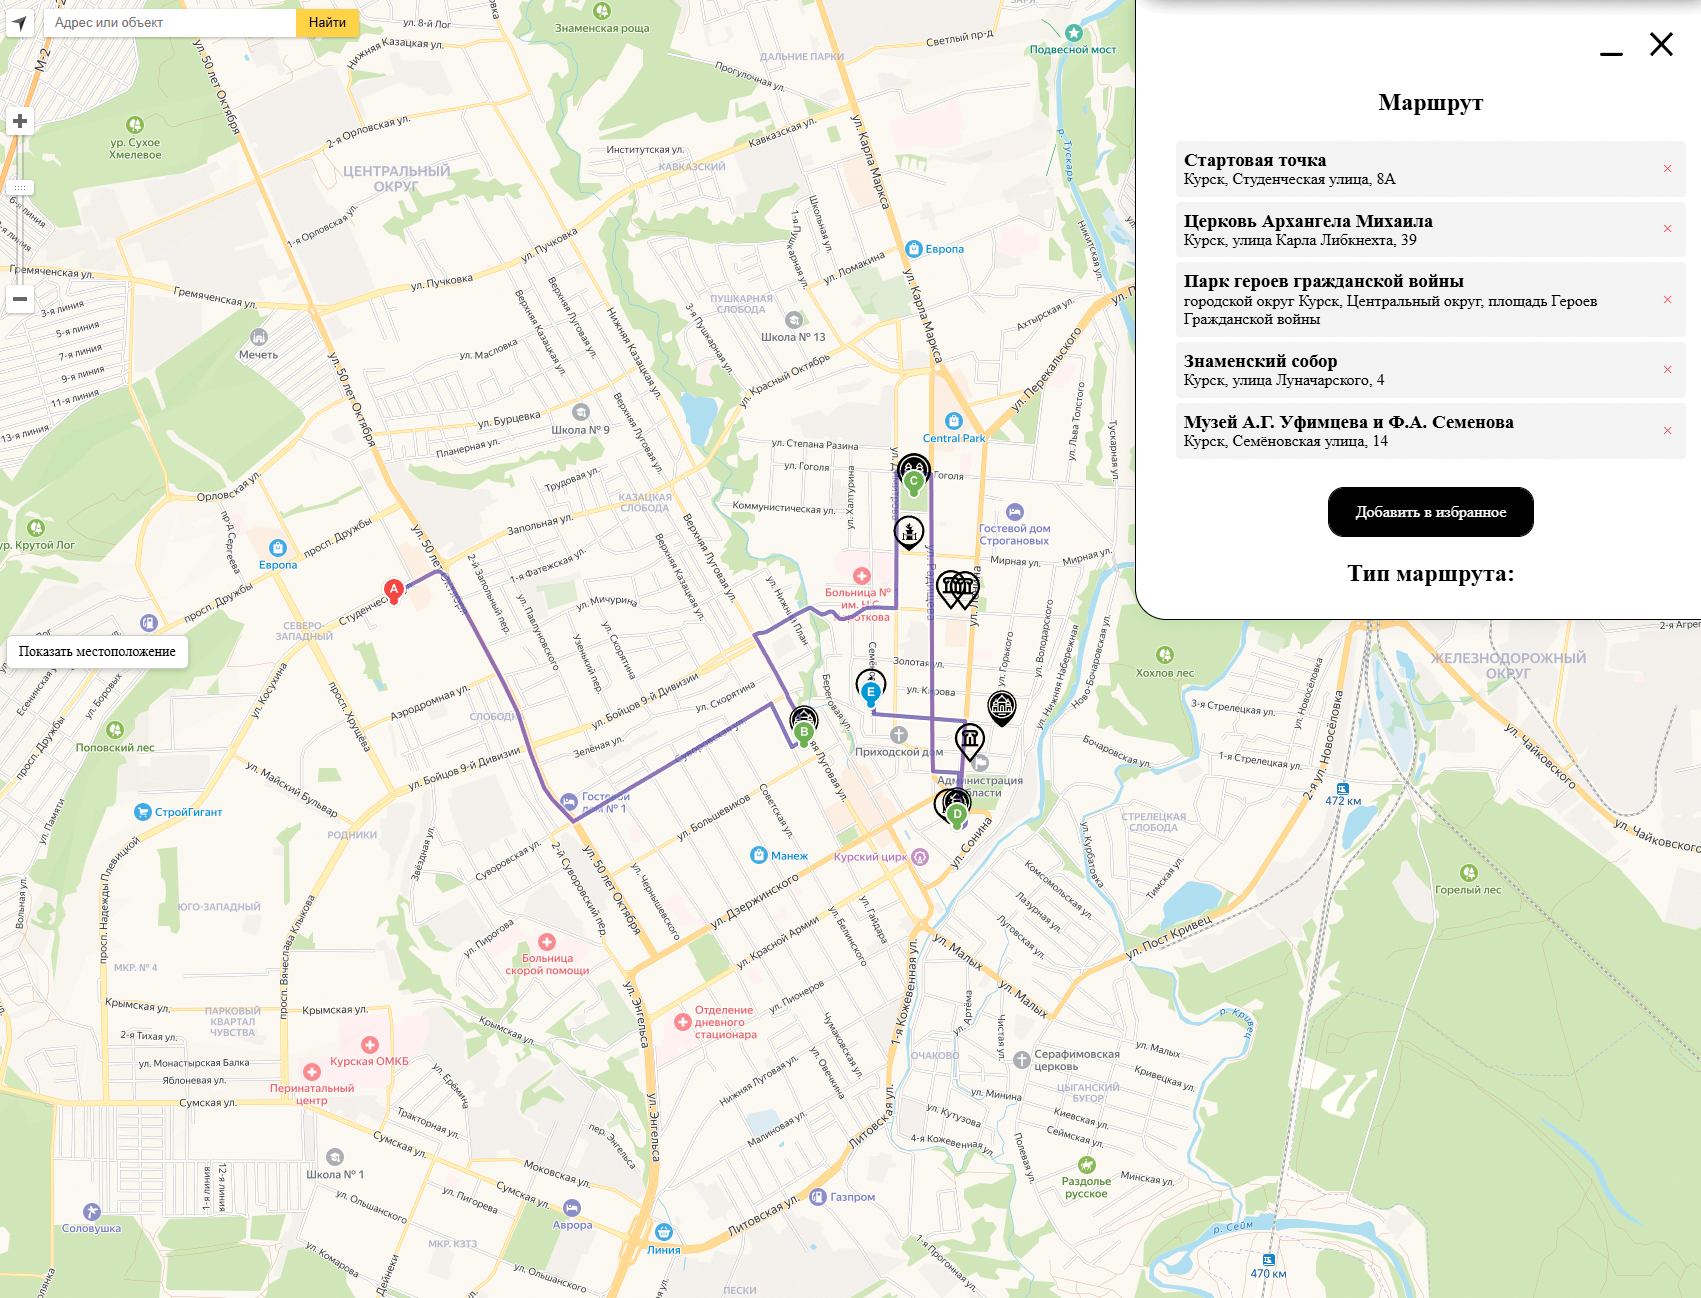
\includegraphics[width=1\linewidth]{r3}}
\caption{Пользовательский маршрут}
\label{r3:image}
\end{figure}

\newpage
На рисунке \ref{r4:image} представлено переключение типа маршрута с автомобильного на пешеходный.

\begin{figure}[H]
	\center{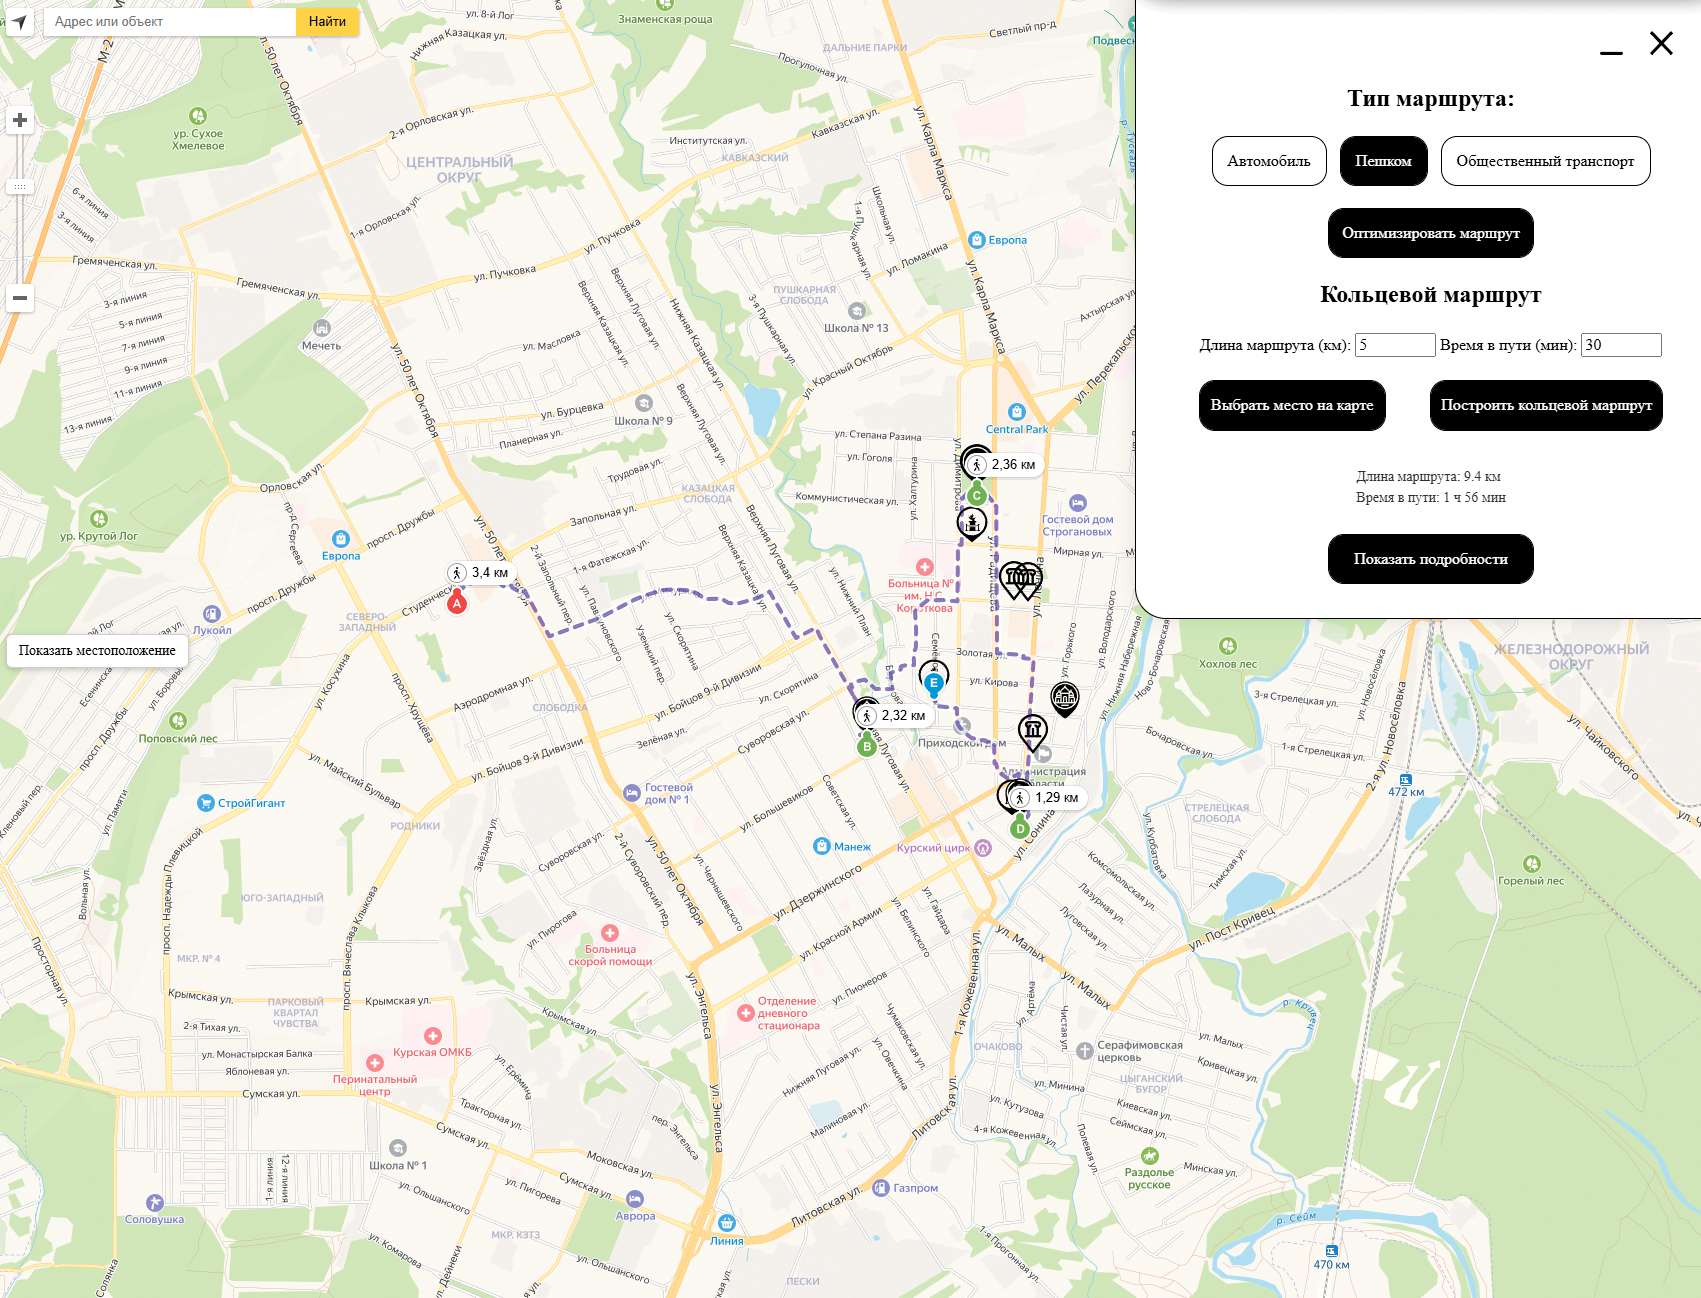
\includegraphics[width=1\linewidth]{r4}}
	\caption{Переключение типа маршрута}
	\label{r4:image}
\end{figure}

\newpage
На рисунке \ref{r11:image} представлена автоматическая оптимизация маршрута.

\begin{figure}[H]
	\center{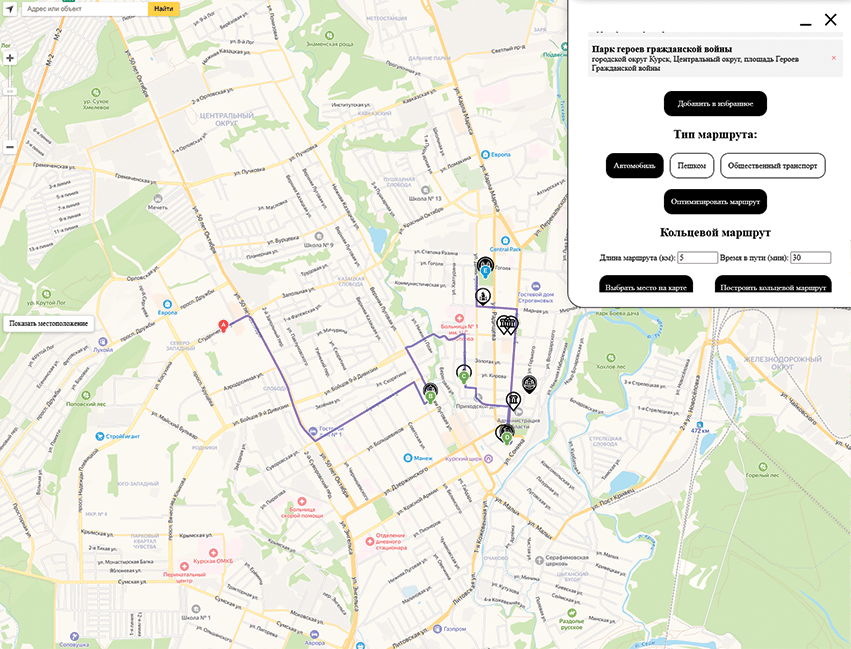
\includegraphics[width=1\linewidth]{r11}}
	\caption{Оптимизированный маршрут}
	\label{r11:image}
\end{figure}

\newpage
На рисунке \ref{r5:image} представлена автоматическая генерацию кольцевого маршрута по указанным пользователем параметрам.

\begin{figure}[H]
	\center{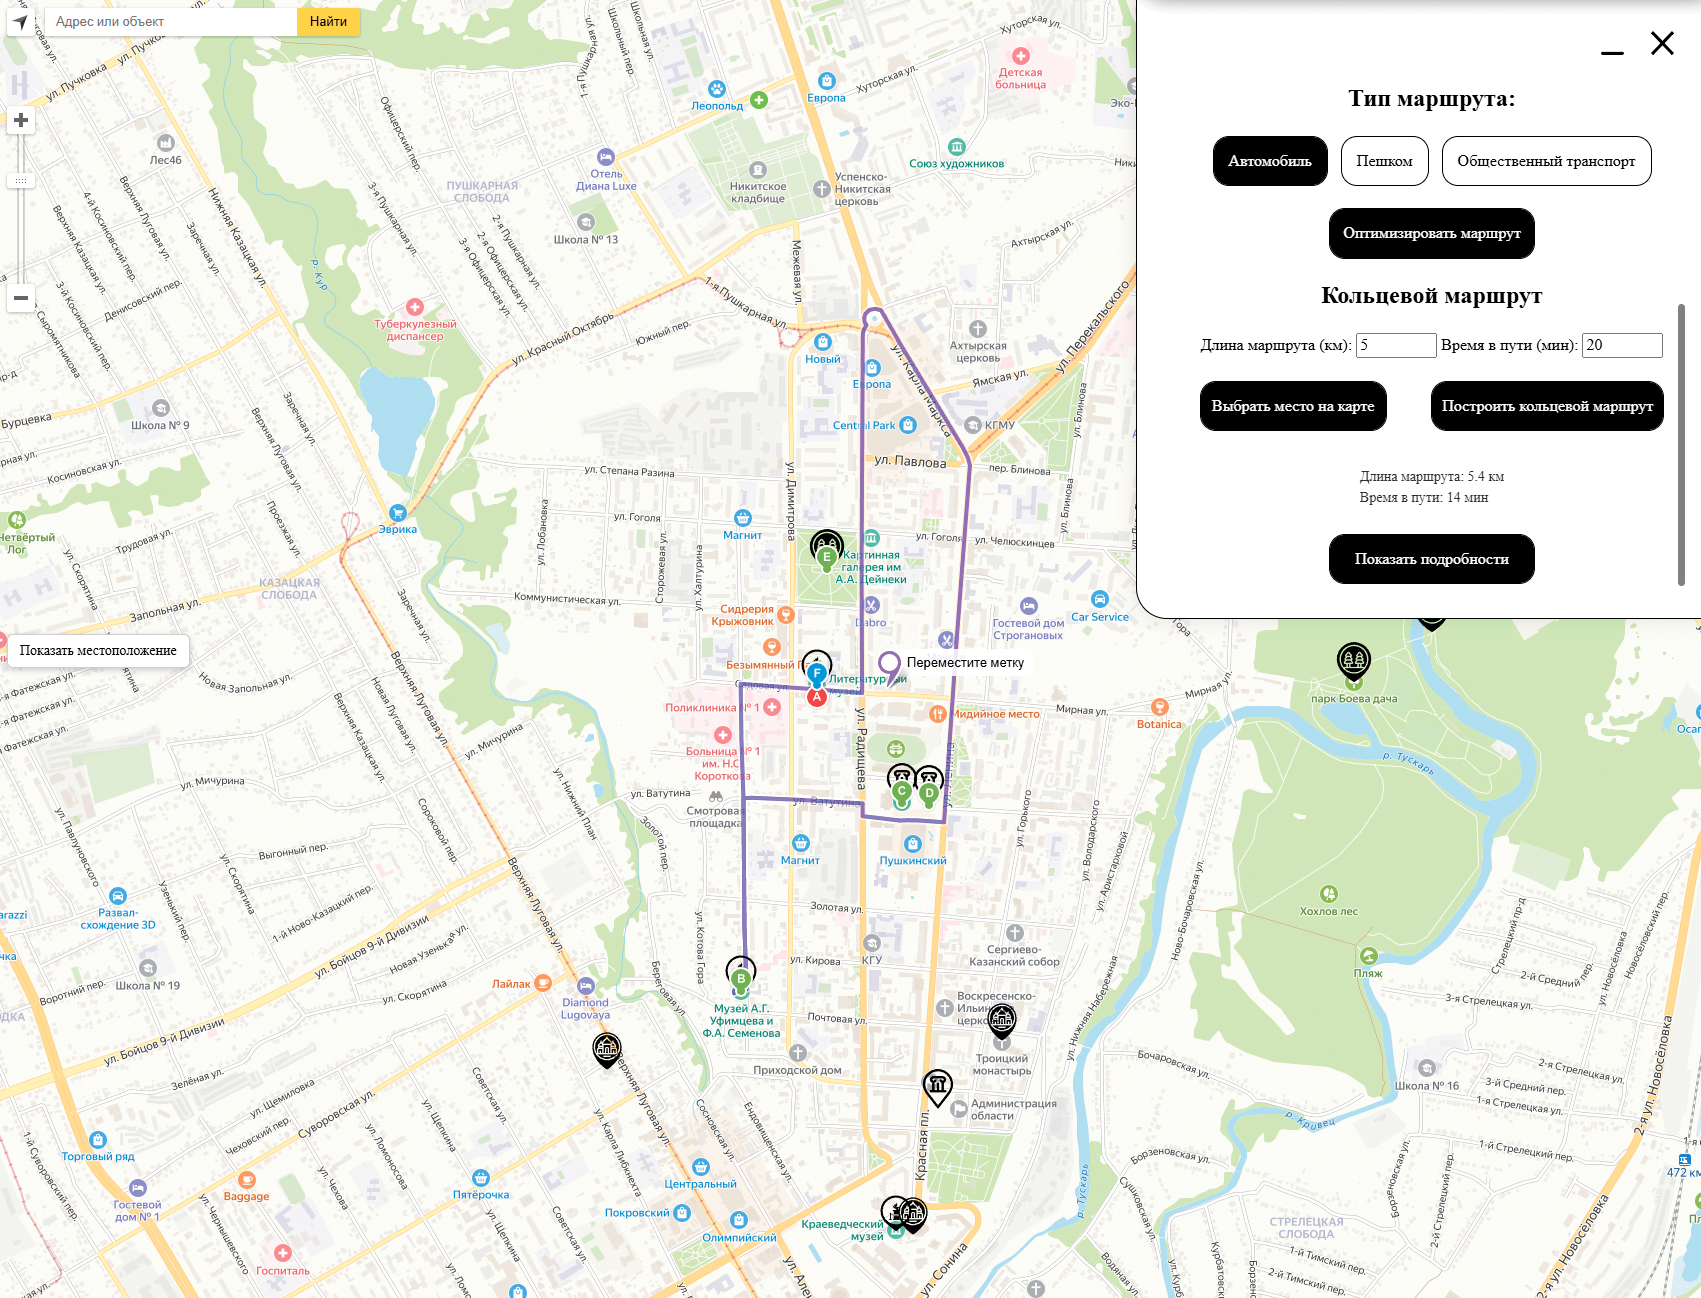
\includegraphics[width=1\linewidth]{r5}}
	\caption{Кольцевой маршрут}
	\label{r5:image}
\end{figure}

\newpage
На рисунке \ref{r6:image} представлена фильтрация объектов на карте.

\begin{figure}[H]
	\center{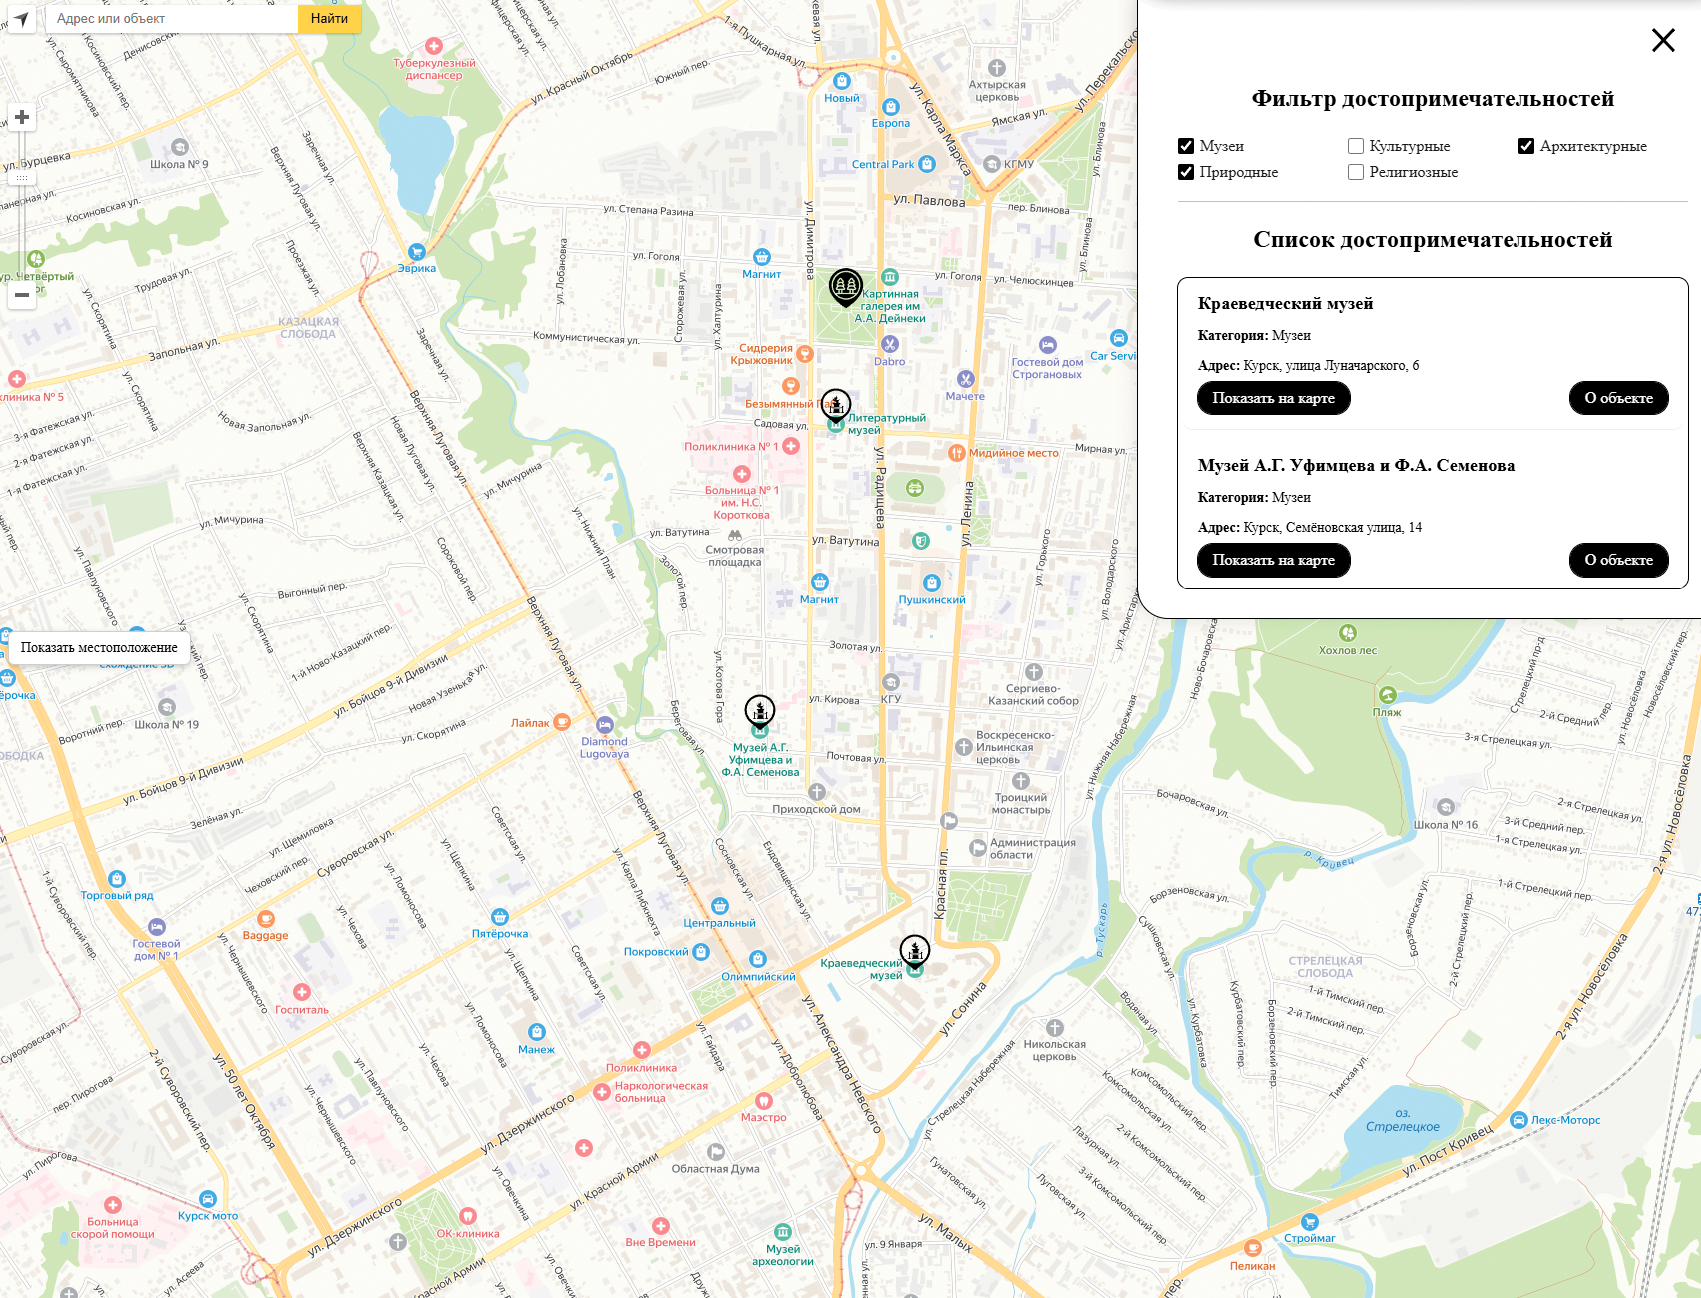
\includegraphics[width=1\linewidth]{r6}}
	\caption{Фильтрация объектов}
	\label{r6:image}
\end{figure}

\newpage
На рисунке \ref{r7:image} представлено определение местоположения пользователя.

\begin{figure}[H]
	\center{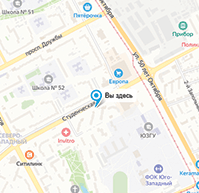
\includegraphics[width=1\linewidth]{r7}}
	\caption{Определение местоположения пользователя}
	\label{r7:image}
\end{figure}

\newpage
На рисунке \ref{r8:image} представлена регистрация нового пользователя.

\begin{figure}[H]
	\center{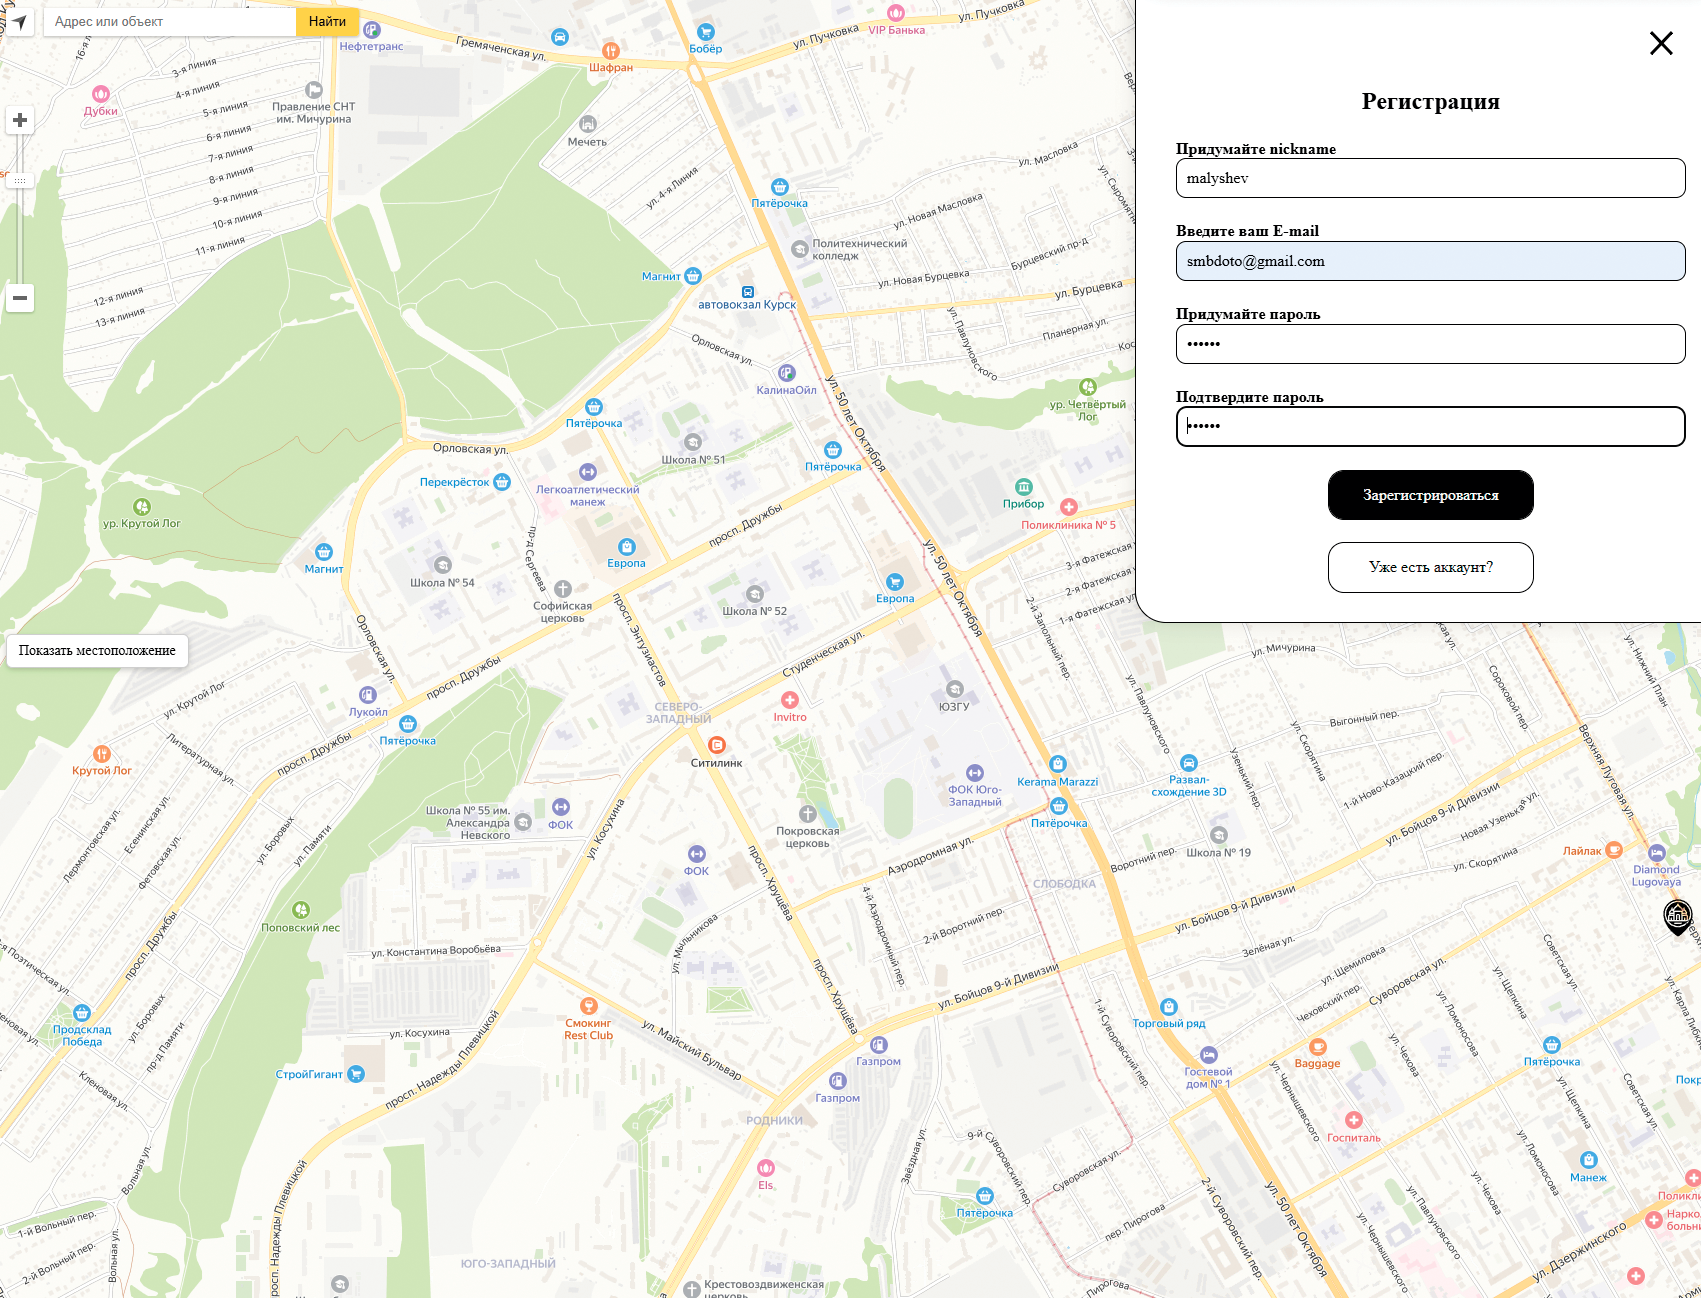
\includegraphics[width=1\linewidth]{r8}}
	\caption{Регистрация пользователя}
	\label{r8:image}
\end{figure}

\newpage
На рисунке \ref{r9:image} представлен вход пользователя в личный кабинет.

\begin{figure}[H]
	\center{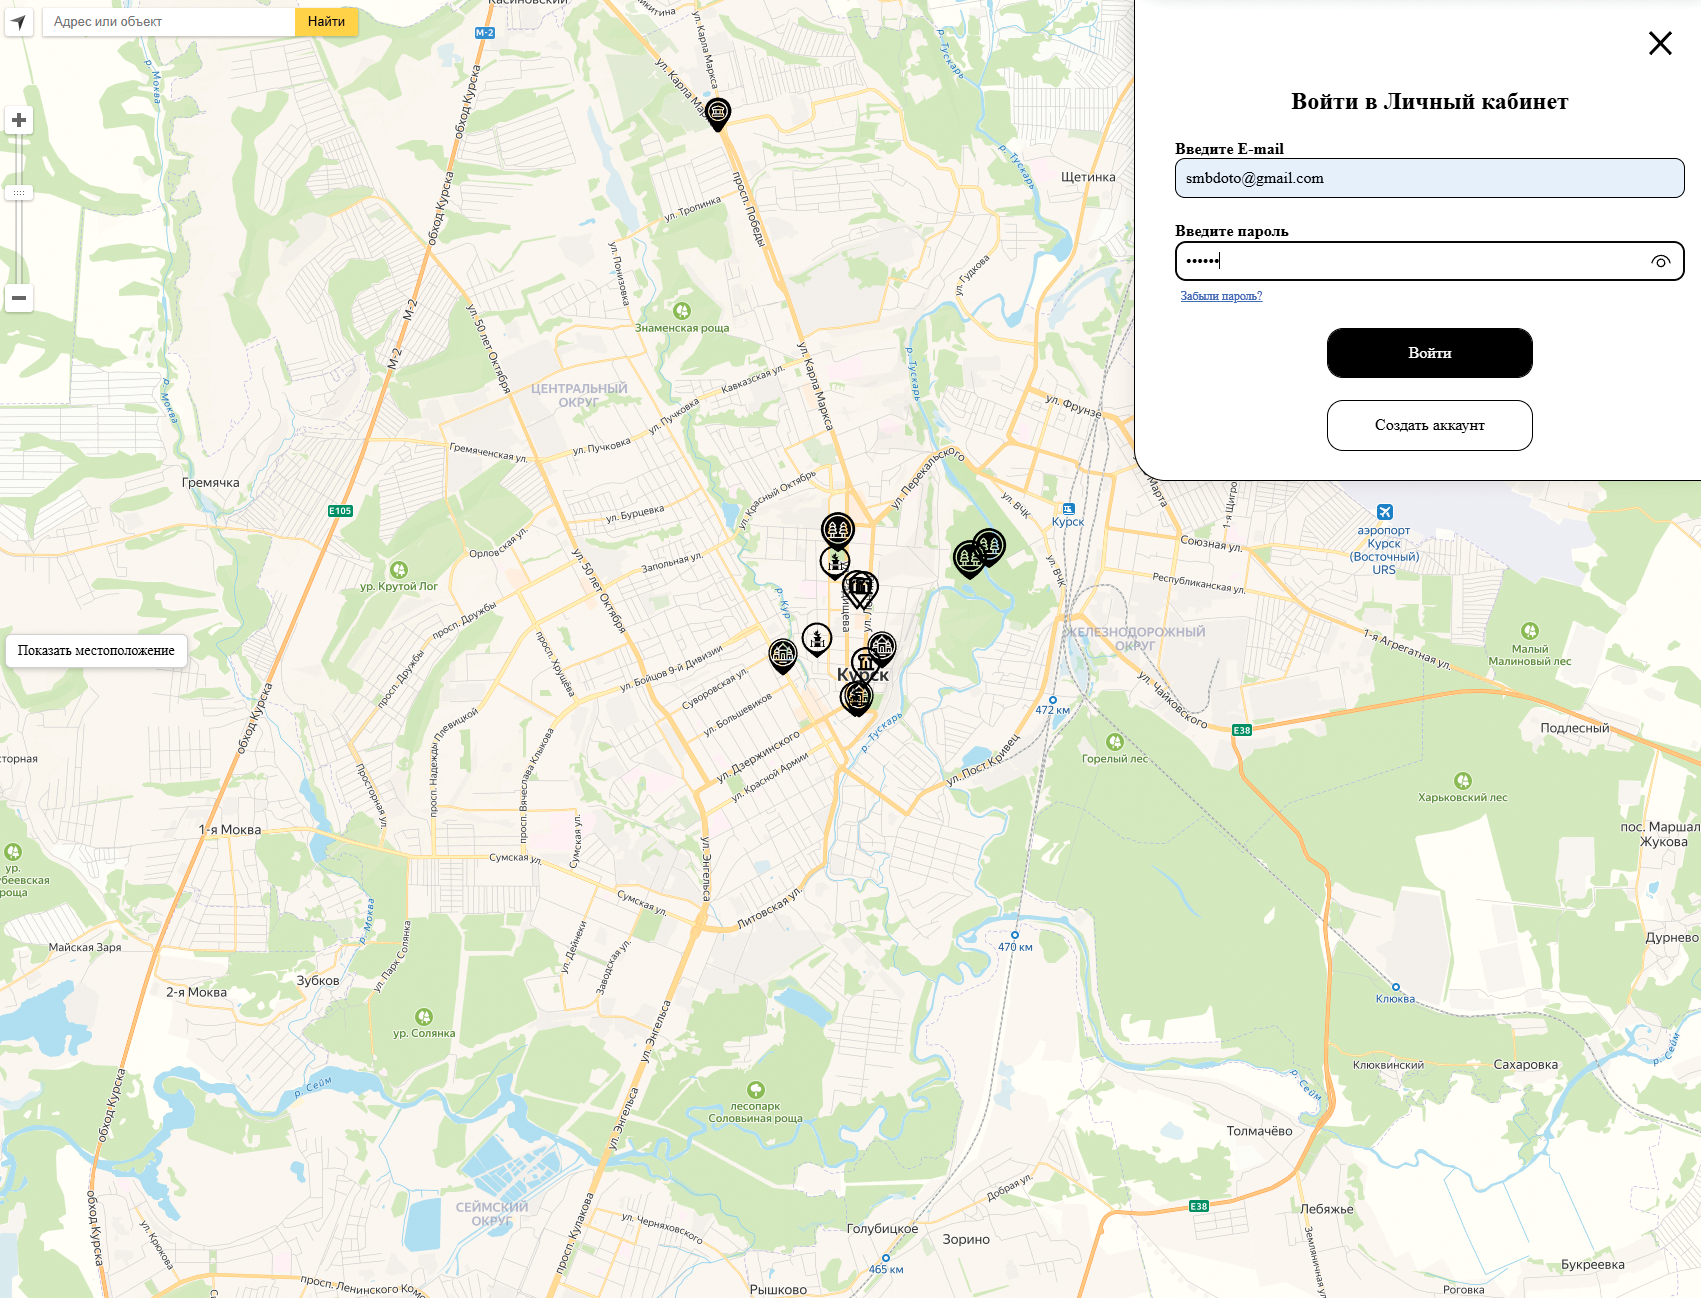
\includegraphics[width=1\linewidth]{r9}}
	\caption{Вход в личный кабинет}
	\label{r9:image}
\end{figure}

\newpage
На рисунке \ref{r10:image} представлено сохранение избранных мест пользователя.

\begin{figure}[H]
	\center{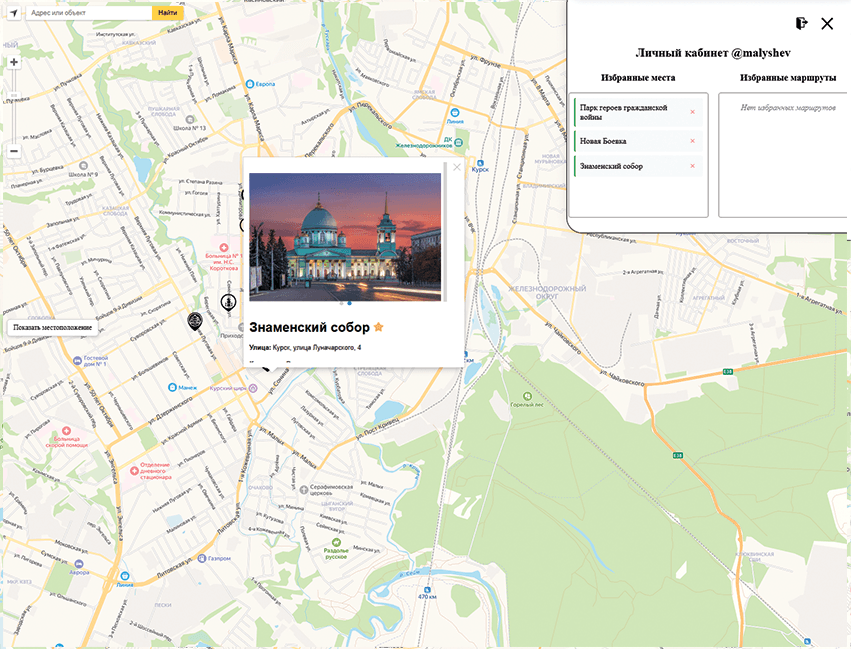
\includegraphics[width=1\linewidth]{r10}}
	\caption{Избранные места}
	\label{r10:image}
\end{figure}

\newpage
На рисунке \ref{r12:image} представлено сохранение избранного маршрута.

\begin{figure}[H]
	\center{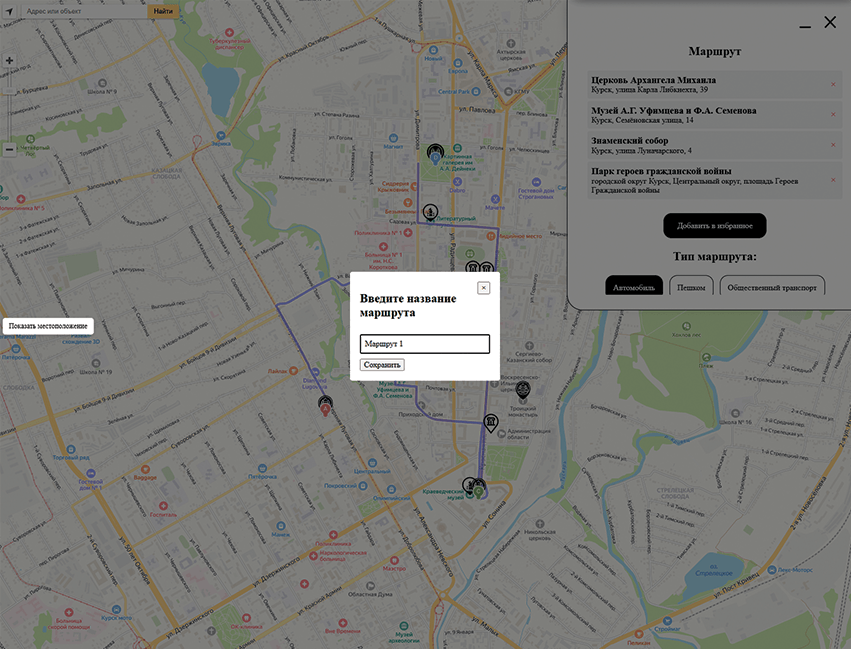
\includegraphics[width=1\linewidth]{r12}}
	\caption{Сохранение маршрута}
	\label{r12:image}
\end{figure}

\newpage
На рисунке \ref{r13:image} представлено отображение маршрута в личном кабинете.

\begin{figure}[H]
	\center{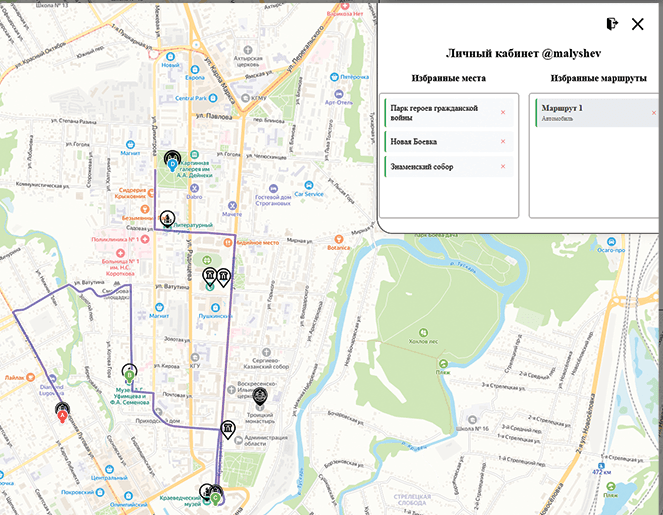
\includegraphics[width=1\linewidth]{r13}}
	\caption{Избранные маршруты}
	\label{r13:image}
\end{figure}

\newpage
На рисунке \ref{r14:image} представлено добавление нового объекта на карту.

\begin{figure}[H]
	\center{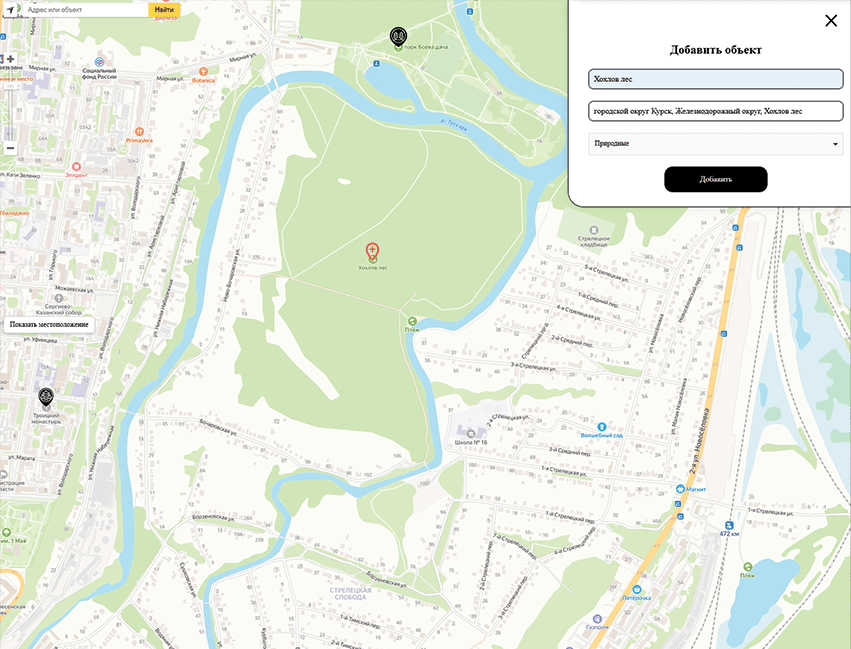
\includegraphics[width=1\linewidth]{r14}}
	\caption{Добавление нового объекта}
	\label{r14:image}
\end{figure}

\newpage
На рисунке \ref{r15:image} представлена проверка нового места администратором.

\begin{figure}[H]
	\center{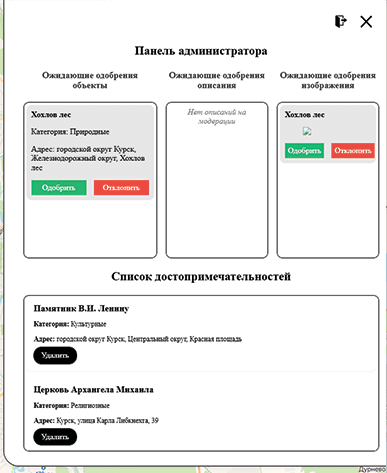
\includegraphics[width=1\linewidth]{r15}}
	\caption{Панель администратора}
	\label{r15:image}
\end{figure}

\newpage
На рисунке \ref{r16:image} представлено появление нового объекта на карте, после одобрения.

\begin{figure}[H]
	\center{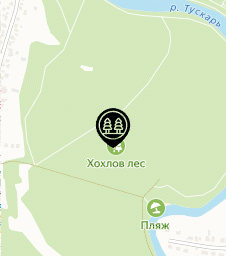
\includegraphics[width=1\linewidth]{r16}}
	\caption{Появление нового объекта на карте}
	\label{r16:image}
\end{figure}

\newpage
На рисунке \ref{r17:image} представлено добавление описания для объекта, если это делает администратор, проверки не требуется.

\begin{figure}[H]
	\center{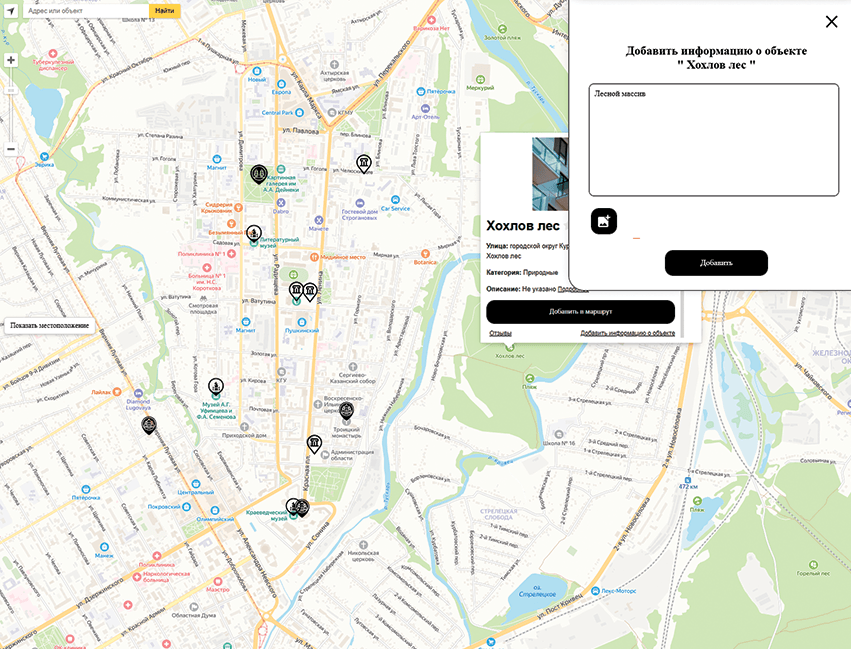
\includegraphics[width=1\linewidth]{r17}}
	\caption{Добавление описания}
	\label{r17:image}
\end{figure}

\newpage
На рисунке \ref{r18:image} представлено новое описание объекта.

\begin{figure}[H]
	\center{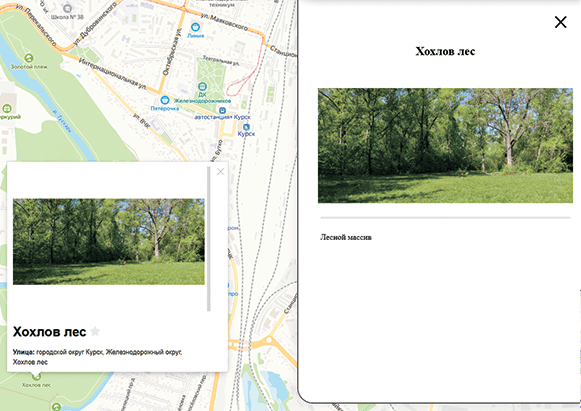
\includegraphics[width=1\linewidth]{r18}}
	\caption{Новое описание объекта}
	\label{r18:image}
\end{figure}

\newpage
На рисунке \ref{r19:image} представлена панель отзывов об объекте.

\begin{figure}[H]
	\center{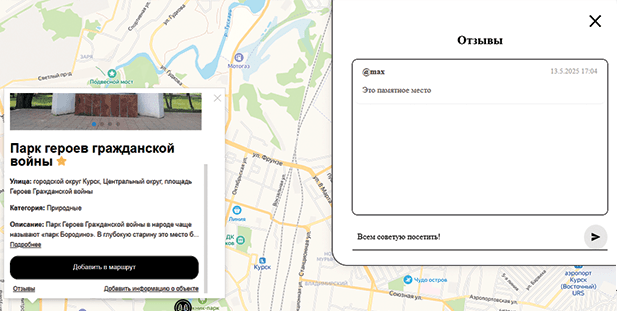
\includegraphics[width=1\linewidth]{r19}}
	\caption{Панель отзывов}
	\label{r19:image}
\end{figure}

\newpage
На рисунке \ref{r20:image} представлено добавление нового отзыва об объекте.

\begin{figure}[H]
	\center{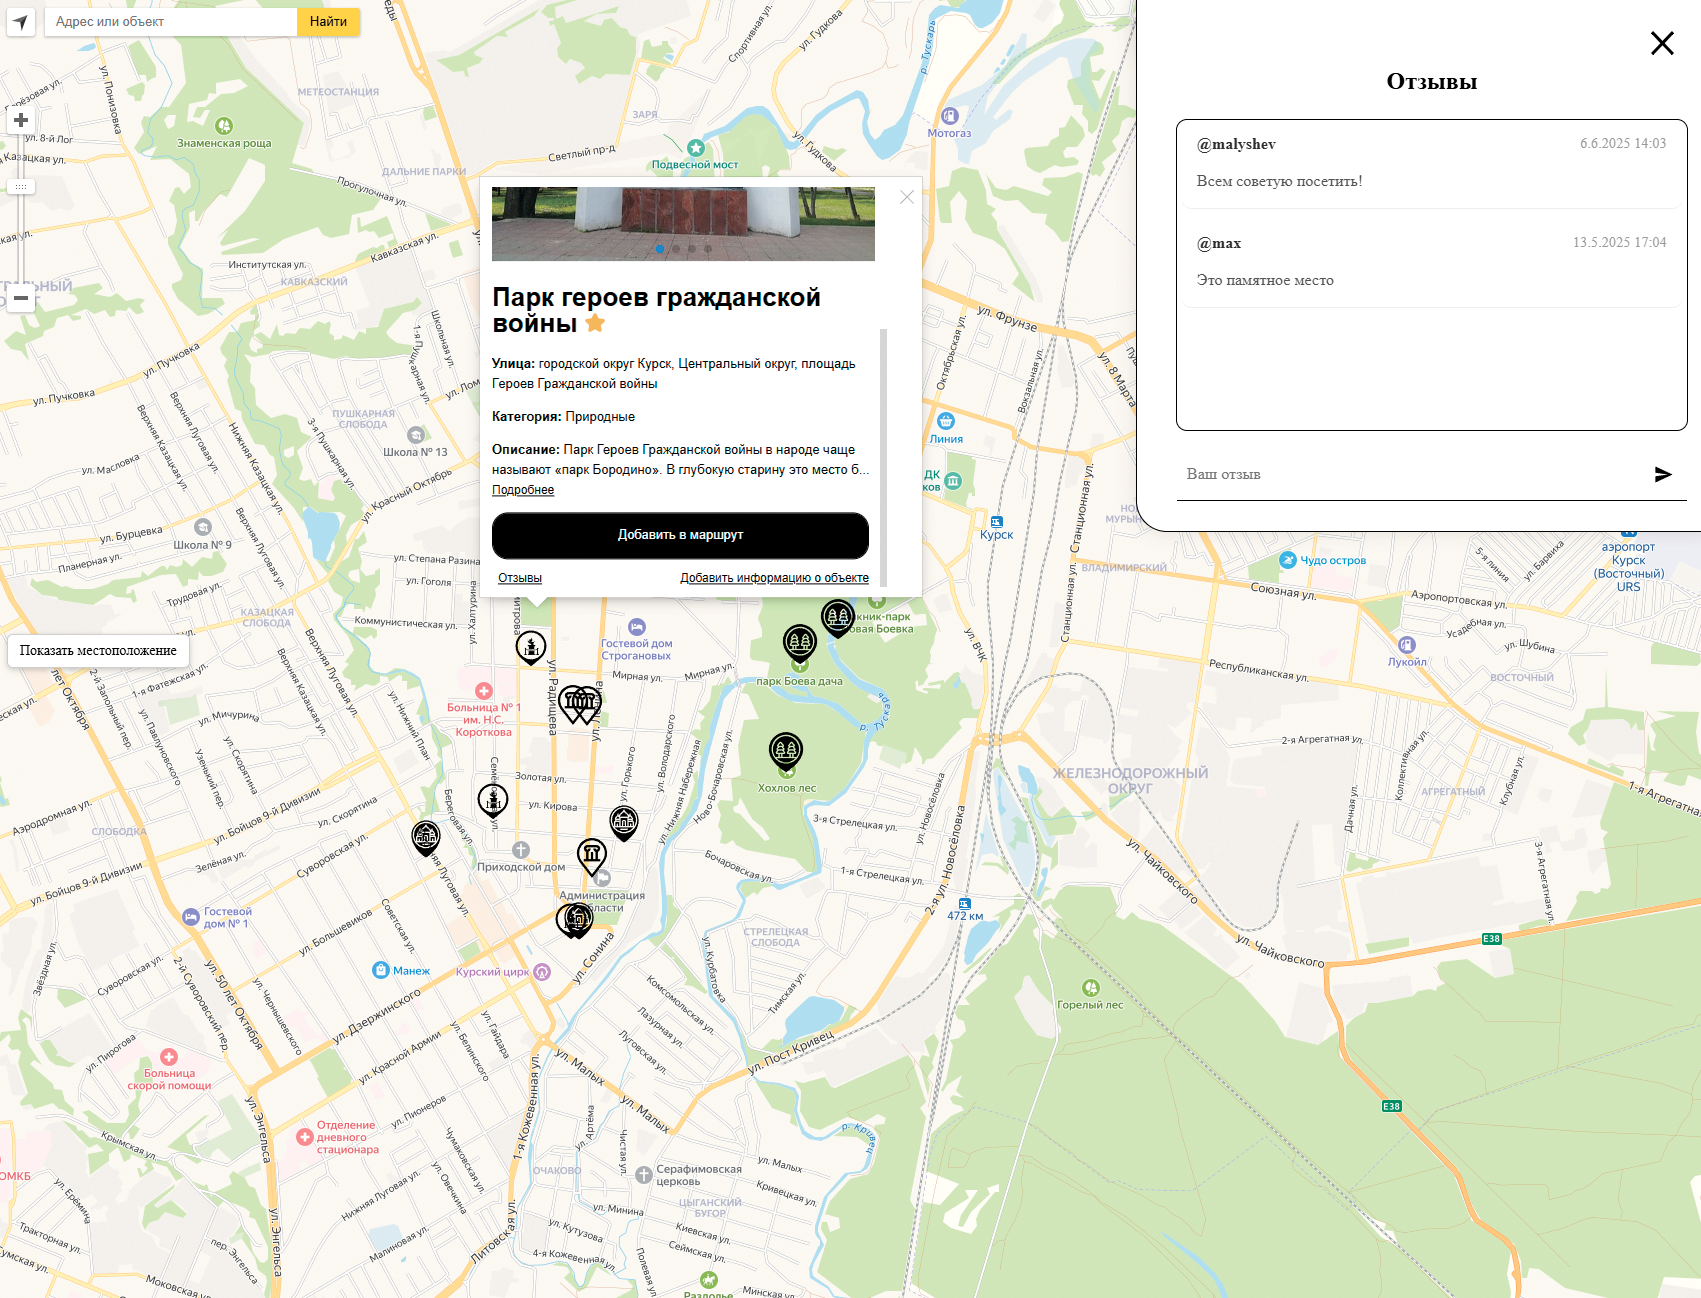
\includegraphics[width=1\linewidth]{r20}}
	\caption{Добавление нового отзыва}
	\label{r20:image}
\end{figure}

\subsection{Сборка компонентов программной системы}

На заключительном этапе разработки осуществляется объединение всех разработанных компонентов в единую, целостную программную систему. Сборка включает настройку взаимосвязей между модулями, интеграцию клиентской и серверной части, подключение внешних API, а также развёртывание проекта в рабочей среде. Этот процесс требует особой внимательности, так как от согласованной работы всех частей напрямую зависит стабильность и надёжность всего приложения.

В рамках настоящего проекта сборка компонентов осуществлялась поэтапно. Сначала были интегрированы скрипты визуализации и взаимодействия с картой, реализованные на JavaScript с использованием API Яндекс.Карт. Далее подключены модули обработки пользовательских данных, включая систему авторизации, добавления объектов, отзывов и избранного. Серверная логика на PHP была связана с клиентскими запросами через интерфейс асинхронного обмена данными, обеспечивая быструю реакцию интерфейса без перезагрузки страницы.

Файловая структура проекта была организована по принципу логического разделения ответственности: отдельные каталоги для стилей, сценариев, изображений и обработчиков данных. Это обеспечило не только удобство сопровождения, но и упростило процесс масштабирования проекта в будущем. Все компоненты, включая формы, фильтры, модальные окна, навигационные панели и маршрутизаторы, были приведены к единому стилю и протестированы на совместимость.

После завершения сборки система была развернута в тестовой среде, где прошла полную проверку функциональности. Успешное объединение клиентской и серверной логики позволило обеспечить полноценную работу всех функций, предусмотренных техническим заданием, включая отображение объектов на карте, взаимодействие с балунами, построение и сохранение маршрутов, а также взаимодействие с пользовательскими данными.

Таким образом, сборка компонентов завершила цикл разработки программной системы и обеспечила её готовность к развертыванию в продуктивной среде.
